\documentclass{article}

\usepackage{amsmath}
\usepackage[german]{babel}
\usepackage{caption}
\usepackage{csquotes}
\usepackage{geometry}
\usepackage{graphicx}
\usepackage{hyperref}
\usepackage{listings}
\usepackage{lmodern}
\usepackage{makecell}
\usepackage{mathtools}
\usepackage{multirow}
\usepackage{scrextend}
\usepackage{tabularx}
\usepackage{titlesec}
\usepackage{arydshln}
\usepackage{xspace}
\usepackage{xurl}

\titlespacing*{\section}
{0pt}{1ex plus 1ex minus .2ex}{0.3ex plus .2ex}
\titlespacing*{\subsection}
{0pt}{1ex plus 1ex minus .2ex}{0.3ex plus .2ex}

\deffootnote{0em}{1.6em}{\thefootnotemark.\enskip}
\setlength{\tabcolsep}{0.1em}
\def\arraystretch{1.2}

\expandafter\def\expandafter\normalsize\expandafter{%
    \normalsize%
    \setlength\abovedisplayskip{0pt}%
    \setlength\belowdisplayskip{0pt}%
    %\setlength\abovedisplayshortskip{-8pt}%
    %\setlength\belowdisplayshortskip{2pt}%
}
%\setlength{\itemsep}{3pt}
%\setlength{\parsep}{3pt}
%\setlength{\topsep}{3pt}

\newcommand{\imgsize}{\texttt{(224, 224, 3)}\xspace}
\newcommand{\resnet}{ResNet50\xspace}
\newcommand{\effnet}{EfficientNetB0\xspace}

\title{Generalizable Deepfake Detection}
\author{Bernhard Birnbaum}

\begin{document}

\maketitle

\section{Aufgabe \& Stand der Technik}\label{sec:introduction}
Im Rahmen des Praktikums \enquote{Implementierung in Forensik und Mediensicherheit} soll ein Modell zur Klassifikation von DeepFake-Bildsequenzen konzeptioniert, implementiert und evaluiert werden.
Mit geeigneten Metriken soll überprüft werden, ob über die Detektion hinaus eine Unterscheidung von verschiedenen DeepFake-Techniken (explizit \textit{face-swap} (\texttt{FS}) und \textit{face-reenactment} (\texttt{FR})) etabliert werden kann.
%\cite{deeplearningbook}
%\footnote{Machine Learning, Google for Developers, \url{https://developers.google.com/machine-learning}}
\\[0.5em]
\textbf{DeepLearning-Architekturen für sequentielle Daten}:\\
Um sequentielle Daten (z.B. Frames eines Videos) zu klassifizieren, werden rekurrente Architekturen genutzt (\textit{recurrent neural networks}, RNNs).
Eine weiterentwickelte Form von RNNs stellen die \textit{long short-term memory networks} (LSTMs) dar, welche durch ihre speziellen Speicherzellen mit Gate-Mechanismen langfristige Abhängigkeiten effizienter lernen können und dabei dazu beitragen, das \textit{vanishing gradients problem} zu reduzieren.
Sogenannte \textit{bidirectional LSTMs} ermöglichen darüber hinaus die Verarbeitung von Bildsequenzen in Vor- und Rückrichtung, was eine verbesserte Erfassung von zeitlichen Kontextinformationen ermöglicht.
% https://medium.com/@anishnama20/understanding-bidirectional-lstm-for-sequential-data-processing-b83d6283befc
\\[0.5em]
\textbf{Merkmalsextraktor als Baseline-Modell}:\\
Das konzeptionierte Modell basiert auf einem Merkmalsextraktor, der einem Fine-Tuning unterzogen wird.
Die während dieser Untersuchung erzeugten Modelle nutzen \textit{convolutional neural networks} (CNNs) als Baseline, um die Komplexität der Eingabedaten zu reduzieren: entweder \resnet oder \effnet.
Beide Architekturen sind besonders gut für die Klassifikation von Bildern geeignet und erzielen dabei State-of-the-Art-Ergebnisse, was sie zu gängigen Merkmalsextraktoren macht.
\resnet~\cite{resnet} nutzt sogenannte \textit{residual connections} bzw. \textit{skip connections}, wodurch die Eingabedaten eine oder mehrere Schichten im Netzwerk überspringen können (wirkt ebenfalls \textit{vanishing gradients problem} entgegen).
%\footnote{Exploring ResNet50: An In-Depth Look at the Model Architecture and Code Implementation, \url{https://medium.com/@nitishkundu1993/exploring-resnet50-an-in-depth-look-at-the-model-architecture-and-code-implementation-d8d8fa67e46f}}
\effnet~\cite{efficientnet} hingegen versucht, die Skalierung von Netzen in Tiefe, Breite und Auflösung zu optimieren (\textit{compound model scaling}), was zu einer deutlichen Verringerung der Anzahl von Parametern führt und dadurch eine besseren Performance bei gleicher Eingabegröße \imgsize ermöglicht.
%\footnote{Understanding EfficientNet - The most powerful CNN architecture, \url{https://arjun-sarkar786.medium.com/understanding-efficientnet-the-most-powerful-cnn-architecture-eaeb40386fad}}
\\[0.5em]
\textbf{Geeigneter Datensatz}:\\
Um eine ausreichende Generalisierung zu erreichen sowie repräsentative Auswertungen durchführen zu können, wird ein breit gestreuter Trainings- bzw. Test-Datensatz benötigt.
Der DF40-Datensatz~\cite{yan2024df40} umfasst DeepFake-Erzeugnisse von 40 verschiedenen Tools inklusive der Originaldaten.
Im Rahmen dieser Arbeit soll in einem ersten Proof-of-Concept zunächst zwischen den Klassen \textit{original} (\texttt{OR}), \textit{face-swap} (\texttt{FS}, 10 Tools) und \textit{face-reenactment} (\texttt{FR}, 13 Tools) unterschieden werden.

\section{Konzept}\label{sec:concept}
\subsection{DF40-Datensatz}\label{ssec:df40}
Da der DF40-Datensatz bereits als vorverarbeitete Version angeboten wird, müssen keine größeren Schritte zur Vorverarbeitung der Daten (wie z.B. \textit{face detection} oder \textit{cropping}) durchgeführt werden.
Dementsprechend haben alle Frames dieselben Abmessungen (\texttt{256x256x3}), allerdings variiert die Länge der einzelnen Sequenzen zwischen 8 und 32.
\\[0.5em]
\textbf{Sequenzlängen-Filterung}:\\
Aus diesem Grund muss bereits im Vorfeld festgelegt werden, mit welcher fixen Sequenzlänge das Modell arbeiten soll.
Deshalb werden alle Sequenzen entweder zugeschnitten (sollten sie zu lang sein) oder aus dem Datenset entfernt (sollten sie zu kurz sein).
Alternativ könnten zu kurze Sequenzen auch mit Padding aufgefüllt werden; da der Datensatz allerdings groß genug ist und nur wenige Sequenzen betroffen sind, wurde darauf verzichtet.
\\[0.5em]
\textbf{Gewichtung der Klassen}:\\
Da die Anzahl von Instanzen pro Klasse im Datensatz nicht gut balanciert sind, werden Klassengewichte (\textit{class weights}) verwendet, um ein ausgeglichenes Training zu ermöglichen.
Desweiteren hängen die tatsächlichen Elementzahlen von der verwendeten Sequenzlänge ab, wie in Tabelle~\ref{tab:df40} dargestellt.
Der Split in Trainings- und Testdaten ist bereits vom Datensatz vorgegeben und wird entsprechend übernommen.
\begin{table}[!h]
    \centering
    \caption{Anzahl Instanzen pro Klasse im Trainings- und Testdatensatz mit Klassengewichten}
    \begin{tabularx}{\textwidth}{|X||c|c|c|c|c|c||c|c|c|}
        \hline
        \multirow{2}{*}{\textbf{Sequenzlänge}} & \multicolumn{3}{c|}{\textbf{Trainingsdaten}} & \multicolumn{3}{c||}{\textbf{Klassengewichte ($\approx$)}} & \multicolumn{3}{c|}{\textbf{Testdaten}} \\\cdashline{2-10}
        & \texttt{OR} & \texttt{FS} & \texttt{FR} & \texttt{OR} & \texttt{FS} & \texttt{FR} & \texttt{OR} & \texttt{FS} & \texttt{FR} \\\hline\hline
        8 Frames  & 999 & 6510 & 8467 & 5.3307 & 0.8180 & 0.6290 & 999 & 7075 & 9423 \\\hline
        12 Frames & 999 & 6509 & 8460 & 5.3280 & 0.8177 & 0.6292 & 999 & 7070 & 9405 \\\hline
        16 Frames & 999 & 6495 & 8445 & 5.3183 & 0.8180 & 0.6291 & 999 & 7058 & 9369 \\\hline
    \end{tabularx}
    \label{tab:df40}
\end{table}
\\[0.5em]
\textbf{Einlesen des Datensatzes}:\\
In Listing~\ref{apx:lst.df40} im Anhang ist die Ordnerstruktur des Datensatzes im \texttt{io/}-Verzeichnis dargestellt.
\begin{enumerate}
    \item\textbf{Durchsuchen der Ordnerstruktur}: Zunächst wird die Ordnerstruktur für jede Klasse nach Elementen durchsucht. Dabei werden die einzelnen \texttt{*.png}-Dateien einer Sequenz anhand ihres Dateinamens sortiert, um die Reihenfolge sicherzustellen. Beim Laden der Elemente wird außerdem die zuvor beschriebene Sequenzlängen-Filterung angewandt.
    \item\textbf{Mischen}: Alle erfassten Items werden anschließend initial auf Pfad-Ebene sortiert, damit eine ausgeglichene Reihenfolge zur Bildung von Batches vorliegt. Außerdem wird der Trainingsdatensatz vor jeder Epoche erneut durchmischt.
    \item\textbf{Preprocessing-Funktion}: Die einzelnen Bilder der Sequenzen (\texttt{256x256x3}) werden decodiert und in Tensoren der Form \imgsize umgewandelt (\textit{resizing}). Bei \resnet muss zudem eine weitere Preprocessing-Funktion verwendet werden, damit das Eingabeformat korrekt ist. Danach werden die Frames entlang der zeitlichen Achse gestapelt (\textit{tensor stacking}). Auf die Labels wird zudem eine One-Hot-Kodierung angewandt.
\end{enumerate}

\subsection{Aufbau des Modells}\label{ssec:model}
Im folgenden wird der grundsätzliche Aufbau des entwickelten Modells beschrieben, mit welchem die Klassifikation durchgeführt wird.
Die einzelnen Schichten sind dabei folgendermaßen charakterisiert:
\begin{enumerate}
    \item\textbf{Input-Layer}:
        In der Eingabeschicht wird die Form des Eingabetensors definiert.
        Diese ergibt sich zum einen aus den Abmessungen eines einzelnen Frames \imgsize, zum anderen aus der Länge der Sequenz, mit der das Modell arbeiten soll.
        \\\textbf{Beispiel} für valide Form einer Eingabe (für Sequenzlänge 12): \texttt{(12, 224, 224, 3)}
    \item\textbf{TimeDistributed-Wrapper mit Merkmalsextraktion}:
        Diese Schicht implementiert die Merkmalsextraktion des Baseline-Modells der zu klassifizierenden Bildsequenz, wahlweise durch \resnet oder \effnet.
        Dabei ist das Ziel, die Eingangsgröße eines jeden Einzelbildes durch Reduktion mit Faltungsschichten und Pooling-Operationen schrittweise zu verkleinern.
        Für jeden Frame \imgsize entsteht dadurch eine Feature-Map der Form \texttt{(7, 7, 2048)} bei \resnet bzw. \texttt{(7, 7, 1280)} bei \effnet.
        Die Merkmale aus der letzten Faltung des Netzwerks werden abschließend mit einem \textit{2d global average pooling} zusammengefasst, wodurch jeder Frame der Sequenz auf einen Tensor der Form \texttt{(2048)} für \resnet bzw. \texttt{(1280)} für \effnet reduziert wird.
        Da die Merkmalsextraktion auf jeden Frame der zu klassifizierenden Bildsequenz parallel angewandt werden muss, wird die Schicht in einem sogenannten TimeDistributed-Wrapper implementiert.
        \\\textbf{Beispiel} für valide Form einer Ausgabe (für Sequenzlänge 12, \resnet): \texttt{(12, 2048)}
        \\\textbf{Beispiel} für valide Form einer Ausgabe (für Sequenzlänge 12, \effnet): \texttt{(12, 1280)}
    \item\textbf{Bidirectional-Wrapper mit LSTM}:
        Die Sequenz von Feature-Maps wird in der nächsten Schicht mit einem LSTM verarbeitet.
        Da das LSTM aus 256 Neuronen besteht und mit Hilfe des Bidirectional-Wrappers in beide Richtungen arbeitet, können insgesamt 512 Merkmalsdimensionenen erfasst werden.
        Desweiteren werden mehrere Maßnahmen gegen Overfitting in das Modell etabliert:
        Zum einen wird auf die Eingaben und rekurrenten Verbindungen der LSTM-Zellen ein Dropout eingeführt, zum anderen wird auf die Gewichte der Eingangsverbindungen und rekurrenten Verbindungen eine L2-Regularisierung angewandt.
        Die Ausgabe des BiLSTM enthält eine verdichtete Darstellung der gesamten Bildsequenz, einschließlich relevanter zeitlicher Abhängigkeiten. 
        \\\textbf{Beispiel} für valide Form einer Ausgabe: \texttt{(512)}
    \item\textbf{Dropout-Layer}:
        Nach der Sequenzverarbeitung wird eine weitere Dropout-Schicht auf die gesamte Ausgabe des BiLSTMs angewandt.
    \item\textbf{Dense-Layer}:
        In einer abschließenden vollständig verbundenen Schicht werden die vom BiLSTM extrahierten Merkmale in die Klassifikationswerte umgewandelt.
        Dabei werden besonders große Gewichte bestraft, indem eine weitere L2-Regularisierung zum Einsatz kommt.
        Für jede Klasse gibt es ein Neuron in der Ausgabeschicht.
        Als Aktivierungsfunktion wird \textit{softmax} genutzt, welche die Rohwerte in Wahrscheinlichkeiten für die Klassen umwandelt, sodass die Summe über alle Neurone der Ausgabe 1 ergibt.
        \\\textbf{Beispiel} für valide Form einer Ausgabe: \texttt{(3)}
\end{enumerate}
In Abbildung~\ref{fig:model} ist der Aufbau des Modell schematisch dargestellt.
\begin{figure}[!h]
    \centering
    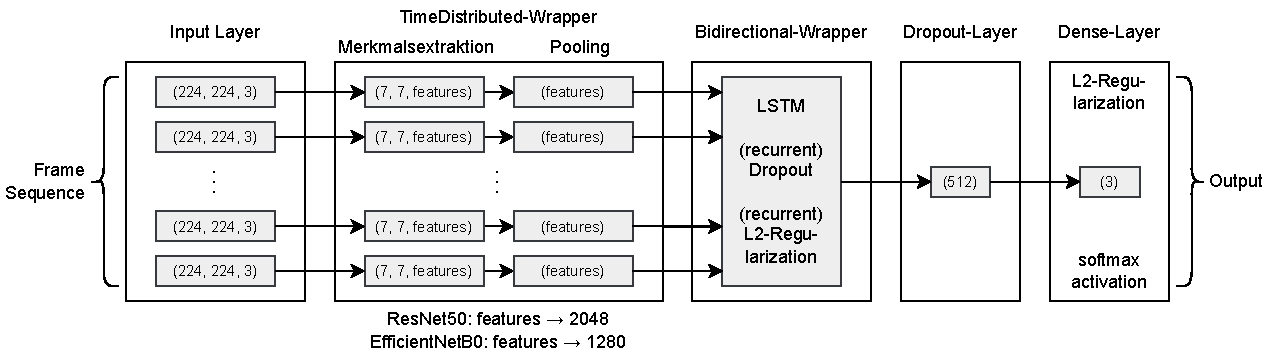
\includegraphics[width=\textwidth]{model.pdf}
    \caption{Schematische Darstellung der Schichten des Modells}
    \label{fig:model}
\end{figure}
    
\subsection{Training}\label{ssec:training}
Im folgenden werden der Ablauf sowie die Parameter des Trainings erläutert.
\\[0.5em]
\textbf{Trainingskonfigurationen}:\\
Insgesamt sollen 6 verschiedene Konfigurationen der Modellarchitektur trainiert werden.
Dabei werden zum einen zwei verschiedene Merkmalsextraktoren als Baseline-Modell getestet (\resnet und \effnet), zum anderen wird die zu klassifizierende Sequenzlänge variiert (8 Frames, 12 Frames, 16 Frames).
Um variierenden den Speicherbedarf durch die verschiedenen Sequenzlängen auszugleichen, wird die Batch-Size entsprechend angepasst (8 Frames $\rightarrow$ 12er Batches, 12 Frames $\rightarrow$ 8er Batches, 16 Frames $\rightarrow$ 4er Batches).
Zur besseren Vergleichbarkeit der Modelle wurde auf \textit{early stopping} verzichtet und alle Konfigurationen werden für exakt 9 Epochen trainiert.
\\[0.5em]
\textbf{Optimierer}:\\
Zum Trainieren wird der Optimizer AdamW verwendet, eine um Weight-Decay erweiterte Variante des Adam-Optimizers (Adaptive Moment Estimation mit L2-Regularisierung).
AdamW verwaltet für jede Gewichtskomponente eine eigene Lernrate, die dynamisch angepasst wird, wodurch auf einen zusätzlichen LR-Scheduler verzichtet werden kann.
\\[0.5em]
\textbf{Verlustfunktion}:\\
Als zu minimierende Verlustfunktion wird \textit{categorical cross-entropy loss} verwendet:
\begin{center}
    $\displaystyle L=-\sum_{i=1}^Cy_i\log(\hat y_i)$ mit Anzahl Klassen $C$, Grundwahrheit $y_i$ und Vorhersage $\hat y_i$
\end{center}
\textbf{Merkmalsextraktoren}:\\
Dem ausgewählten Merkmalsextraktor (\resnet bzw. \effnet) werden initial vortrainierte Gewichte via \texttt{imagenet}~\footnote{ImageNet, \url{https://www.image-net.org/}} zugewiesen.
In den ersten 3 Epochen des Trainings wird er einem Fine-Tuning unterzogen.
Die Anzahl von Schichten, deren Gewichte für das Training freigegeben werden sollen, wird mit folgender Formel berechnet:
\[
    u_i= 
    \begin{dcases}
        \Big\lceil\frac{d}{2^{(2+i)}}\Big\rceil & \text{if } 0\le i \le 2 \\
        0 & \text{otherwise}
    \end{dcases}
    \text{ für Epoche $i$ und Tiefe des Merkmalsextraktors $d$}
\]
\\[0.5em]
\textbf{Lernrate}:\\
Die Größe der Lernrate wird basierend auf $\lambda=0.001$ nach folgender Vorschrift gesetzt:
\[
    \lambda_i= 
    \begin{dcases}
        \frac{\lambda}{10\cdot 2^i} & \text{if } 0\le i \le 2 \\
        \max(\frac{\lambda}{2^i}, 1\cdot 10^{-5}) & \text{otherwise}
    \end{dcases}
    \text{ für Epoche $i$ und Lernrate $\lambda$}
\]
\\Somit ergeben sich die Parametrisierungen und damit die vollständige Trainingskonfiguration für alle 9 Epochen, wie in Tabelle~\ref{tab:layers} dargestellt.
\begin{table}[!h]
    \centering
    \caption{Keras-Schichten für Fine-Tuning der Merkmalsextraktoren und Lernrate pro Epoche}
    \begin{tabularx}{\textwidth}{|X||c|c||c|}
        \hline
        \textbf{Epoche} & \textbf{\resnet ($d=176$)} & \textbf{\effnet ($d=239$)} & \textbf{Lernrate ($\lambda=0.001$)} \\\hline\hline
        Epoche 1 & $u_0=44$ (25\%) & $u_0=60$ (25\%) & $\lambda_0=1\cdot 10^{-4}$ \\\hline
        Epoche 2 & $u_1=22$ (12.5\%) & $u_1=30$ (12.5\%) & $\lambda_1=5\cdot 10^{-5}$ \\\hline
        Epoche 3 & $u_2=11$ (6.25\%) & $u_2=15$ (6.25\%) & $\lambda_2=2.5\cdot 10^{-5}$ \\\hline
        Epoche 4 & \multirow{6}{*}{$u_i=0$ (n.a.)} & \multirow{6}{*}{$u_i=0$ (n.a.)} & $\lambda_3=1.25\cdot 10^{-4}$ \\\cline{1-1}\cline{4-4}
        Epoche 5 &  &  & $\lambda_4=6.25\cdot 10^{-5}$ \\\cline{1-1}\cline{4-4}
        Epoche 6 &  &  & $\lambda_5=3.125\cdot 10^{-5}$ \\\cline{1-1}\cline{4-4}
        Epoche 7 &  &  & $\lambda_6=1.5625\cdot 10^{-5}$ \\\cline{1-1}\cline{4-4}
        Epoche 8 &  &  & $\lambda_7=1\cdot 10^{-5}$ \\\cline{1-1}\cline{4-4}
        Epoche 9 &  &  & $\lambda_8=1\cdot 10^{-5}$ \\\hline
    \end{tabularx}
    \label{tab:layers}
\end{table}
\subsection{Validierung}\label{ssec:validation}
Neben den Testdaten (siehe Tabelle~\ref{tab:df40}) werden für eine aussagekräftige Evaluation geeignete Metriken benötigt.
Diese müssen für Multi-Klassen-Probleme geeignet sein und insbesondere mit unausgewogenen Klassen umgehen können.
\\[0.5em]
\textbf{Precision}: Misst den Anteil der korrekt vorhergesagten positiven Instanzen im Verhältnis zu allen Instanzen, die als positiv vorhergesagt wurden:
    \begin{center}
        $\displaystyle P_i=\frac{\text{TP}_i}{(\text{TP}_i+\text{FP}_i)}$ bzw. $\displaystyle P_\text{micro}=\frac{\sum_{i=1}^C\text{TP}_i}{\sum_{i=1}^C(\text{TP}_i+\text{FP}_i)}$ (aggregierter Durchschnittswert)
    \end{center}
\textbf{Recall}: Misst den Anteil der korrekt vorhergesagten positiven Instanzen im Verhältnis zu allen tatsächlichen positiven Instanzen.
    \begin{center}
        $\displaystyle R_i=\frac{\text{TP}_i}{(\text{TP}_i+\text{FN}_i)}$ bzw. $\displaystyle R_\text{micro}=\frac{\sum_{i=1}^C\text{TP}_i}{\sum_{i=1}^C(\text{TP}_i+\text{FN}_i)}$ (aggregierter Durchschnittswert)
    \end{center}
\textbf{F1-Score}: Ist das harmonische Mittel von Precision und Recall und bietet eine ausgewogene Metrik für die Modellleistung. Bei unbalancierten Daten erhalten Klassen mit mehr Instanzen ein höheres Gewicht.
    \begin{center}
        $\displaystyle F_i=\frac{2\cdot P_i\cdot R_i}{P_i+R_i}$ bzw. $\displaystyle F_\text{weighted}=\frac{\sum_{i=1}^Cw_i\cdot F_i}{\sum_{i=1}^Cw_i}$ mit $w_i=\frac{\text{\#Instanzen Klasse }i}{\text{\#Instanzen gesamt}}$
    \end{center}

\section{Implementierung}\label{sec:implementation}
Das in dieser Untersuchung entwickelte Modell (siehe Abs.~\ref{ssec:model}) wurde mit TensorFlow in Python implementiert.
Als Paket- und Umgebungsmanagement wurde MiniForge mit Mamba verwendet.
Die folgenden Tools bzw. Versionen müssen in der virtuellen Umgebung installiert sein:
\begin{itemize}
    \item Python 3.12.9
    \item tensorflow 2.18.0
    \item numpy 2.0.2
    \item keras 3.8.0
    \item NVIDIA CUDA 12.5.82
\end{itemize}
\textbf{PyTorch vs. TensorFlow}:\\
Für die Implementierung des Modells wurden die beiden ML-Frameworks PyTorch und TensorFlow betrachtet:
\\
PyTorch ist sehr dynamisch bzw. erweiterbar und deshalb für Forschung und Experimente prinzipiell geeignet.
Durch die flexiblen Nutzungsmöglichkeiten ergibt sich allerdings auch eine steilere Lernkurve.
Der Einsatz von PyTorch ist deshalb vor allem dann sinnvoll, wenn mehr Kontrolle über das Modell(training) benötigt wird.
\\
TensorFlow hingegen bietet durch die große Anzahl von High-Level-Schnittstellen und die umfangreiche Dokumentation einen einfacheren Einstieg.
Es ist zudem sehr gut dazu geeignet, mit wenig Code einen lauffähigen Prototypen mit automatischen Optimierungen zu erstellen.
Da im Rahmen dieser Arbeit keine neuen Komponenten für Netze entwickelt werden, sondern lediglich bereits bestehende zu einem neuen Modell kombiniert werden, und zuden wenig praktisches Vorwissen vorhanden war, ist TensorFlow als Framework die bessere Wahl.

\section{Evaluation}
Insgesamt wurden 6 Modellkonfigurationen für jeweils 9 Epochen trainiert (siehe Abs.~\ref{ssec:training}). 
Mit den in Abs.~\ref{ssec:validation} aufgeführten Metriken ergeben sich die folgenden Zahlen zur Performance der Modelle:
\begin{table}[!h]
    \scriptsize
    \centering
    \caption{Auswertung der Klassifikationsergebnisse nach 9 Epochen Training}
    \begin{tabularx}{\textwidth}{|X|c|c|c|c|c|c|c|c|c|c|c|c|c|}
        \hline
        \multirow{2}{*}{\makecell[l]{\textbf{Modellkonfiguration}\\(FE-Sequenzlänge)}} & \multirow{2}{*}{\makecell{\textbf{Zeit}\\pro Item}} & \multicolumn{4}{c|}{\textbf{Precision}} & \multicolumn{4}{c|}{\textbf{Recall}} & \multicolumn{4}{c|}{\textbf{F1-Score}} \\\cdashline{3-14}
        & & \texttt{OR} & \texttt{FS} & \texttt{FR} & micro & \texttt{OR} & \texttt{FS} & \texttt{FR} & micro & \texttt{OR} & \texttt{FS} & \texttt{FR} & weighted \\\hline\hline
        \resnet-08 &  $\text{ms}$ &  &  &  &  &  &  &  &  &  &  &  &  \\\hline
        \resnet-12 &  $\text{ms}$ &  &  &  &  &  &  &  &  &  &  &  &  \\\hline
        \resnet-16 &  $\text{ms}$ &  &  &  &  &  &  &  &  &  &  &  &  \\\hline
        \effnet-08 & 38 $\text{ms}$ & 0.7099 & 0.9049 & 0.8433 & 0.8531 & 0.9920 & 0.7422 & 0.9150 & 0.8531 & 0.8230 & 0.8174 & 0.8782 & 0.8505 \\\hline
        \effnet-12 &  $\text{ms}$ &  &  &  &  &  &  &  &  &  &  &  &  \\\hline
        \effnet-16 &  $\text{ms}$ &  &  &  &  &  &  &  &  &  &  &  &  \\\hline
    \end{tabularx}
    \label{tab:evaluation}
\end{table}
\begin{itemize}
    \item \textbf{ToDo}: Metriken und Detektionszeiten erfassen und eintragen
    \item \textbf{ToDo}: Auswertung/Bewertung
\end{itemize}

\section{Zusammenfassung}
\subsection{Fazit}
\begin{itemize}
    \item \textbf{ToDo}: Fazit \dots
\end{itemize}

\subsection{Ausblick für zukünftige Arbeiten}
\textbf{Weitere Klassen}:\\
Im DF40-Datensatz sind neben \textit{face-swap}- und \textit{face-reenactment}-Sequenzen auch Erzeugnisse von \textit{entire face synthesis}- oder \textit{face edit}-Tools vorhanden.
In einer weiterführenden Untersuchung kann geprüft werden, ob die Modelle auch für 4 bzw. 5 Klassen ausreichend gute Ergebnisse erzielen.
\\[0.5em]
\textbf{Vision Transformer als Merkmalsextraktor}:\\
Die entwickelten Modelle nutzen aktuell beide CNN-Architekturen, entweder \resnet oder \effnet als Baseline-Klassifikator.
Vision Transformer stellen einen alternativen Ansatz zur Merkmalsextraktion mittels \textit{self attention} dar.
In einer weiterführenden Arbeit könnte ein entsprechend angepasstes Transformer-Modell mit der Performance der Modelle dieser Arbeit verglichen werden.  
\\[0.5em]
\textbf{Data Augmentation}:\\
In dieser Arbeit wurden Klassengewichte genutzt, um unausgewogene Klassen zu balancieren.
Alternativ könnte mit einer Datenaugmentation eine fortgeschrittene Oversampling-Technik eingesetzt werden, um zusätzliche Datenpunkte zu erstellen.
Eine gute Datenaugmentation hat das Potenzial, das Generalisierungsvermögen der Modelle weiter zu steigern.
\\[0.5em]
\textbf{Zusätzliche Validierungsdaten}:\\
Der DF40-Datensatz wird zwar bereits mit einem Validierungssplit ausgeliefert, allerdings sollte noch mindestens ein weiteres Datenset (z.B. DeepSpeakV1~\footnote{DeepSpeakV1, \url{https://huggingface.co/datasets/faridlab/deepspeak_v1}}) hinzugezogen werden, um die Generalisierung auf einer breiteren Datenbasis zu bestätigen.
\\[0.5em]
\textbf{Erweiterte Vorverarbeitung}:\\
Das Modell kann aktuell nur Bildsequenzen mit Framegröße \imgsize klassifizieren.
Deshalb sollte in Framework um das Modell herum implementiert werden, welches geeignete Frames zunächst aus einem zu überprüfenden Video extrahiert (\textit{face detection}) und zuschneidet (\textit{cropping}).
Erst mit der extrahierten Sequenz kann das Modell praktisch genutzt werden.
\\[0.5em]
\textbf{Auflösung erhöhen}:\\
Zu guter Letzt verarbeiten die aktuell verwendeten Merkmalsextraktoren \resnet und \effnet Bilder der Größe \imgsize.
Da die Bilder im DF40-Datensatz eine Größe von \texttt{256x256x3} haben, gehen durch die \textit{resizing}-Operation einige Informationen verloren.
Durch die Verwendung gesteigerter Netztiefen und -breiten könnten die Ergebnisse eventuell weiter verbessert werden.

\newpage
\bibliographystyle{plain}
\bibliography{refs}

\section*{Anhang}
\begin{lstlisting}[label={apx:lst.df40},caption={Ordnerstruktur des DF40-Datensets im \texttt{io/}-Verzeichnis}]
df40/
    test/
        original/
            ffpp/frames/
                <item>/*.png
        face_swap/
            <tool>/frames/
                <item>/*.png
        face_reenact/
            <tool>/frames/
                <item>/*.png
    train/
        original/
            ffpp/frames/
                <item>/*.png
        face_swap/
            <tool>/frames/
                <item>/*.png
        face_reenact/
            <tool>/frames/
                <item>/*.png
\end{lstlisting}

\end{document}
